%\documentclass[hyperref={pdfpagelabels=false},slidetop,9pt]{beamer}
\documentclass[slidetop,8pt]{beamer}
\usepackage[T1]{fontenc}
\usepackage[utf8]{inputenc}
\newcommand{\id}{54}
\newcommand{\nom}{Liaisons mécaniques}
\newcommand{\sequence}{04}
\newcommand{\num}{01}
\newcommand{\type}{TP}
\newcommand{\descrip}{Modélisation d'un solide. Comportement des liaisons mécaniques. Modéliser les mécanismes du laboratoire par un schéma cinématique, paramétré.}
\newcommand{\competences}{A3-C4: Analyse d'architecture et de comportement \\ &  Mod1-C1: Isolement d'un solide ou d'un système de solides \\ &  Mod2-C10-1: Modèle de solide indéformable \\ &  Mod2-C11: Modélisation géométrique et cinématique des mouvements entre solides indéformables \\ &  Mod2-C12: Modélisation cinématique des liaisons entre solides \\ &  Mod2-C15: Modélisation des actions mécaniques \\ &  Rés-C6: Utilisation d'un solveur ou d'un logiciel multi physique \\ &  Com1-C1: Différents descripteurs introduits dans le programme \\ &  Com2-C4: Outils de communication}
\newcommand{\nbcomp}{9}
\newcommand{\systemes}{Plateforme Stewart}
\newcommand{\systemessansaccent}{Plateforme Stewart}
\newcommand{\ilot}{2}
\newcommand{\ilotstr}{02}
\newcommand{\dossierilot}{\detokenize{Ilot_02 Plateforme Stewart}}
\newcommand{\imageun}{Plateforme}

\newcommand{\urlsysteme}{\href{https://www.costadoat.fr/systeme/57}{Ressources système}}
\newcommand{\matlabsimscape}{\href{https://github.com/Costadoat/Sciences-Ingenieur/raw/master/Systemes/Plateforme Stewart/Plateforme_Stewart_Simscape.zip}{Modèle Simscape}}
\newcommand{\solidworks}{\href{https://github.com/Costadoat/Sciences-Ingenieur/raw/master/Systemes/Plateforme Stewart/Plateforme_Stewart_Solidworks.zip}{Modèle Solidworks}}
\newcommand{\edrawings}{\href{https://github.com/Costadoat/Sciences-Ingenieur/raw/master/Systemes/Plateforme Stewart/Plateforme_Stewart.EASM}{Modèle eDrawings}}
\newcommand{\test}{Stewart_param1}
\newcommand{\testi}{Stewart_param2}
\newcommand{\testii}{Stewart_param3}
\newcommand{\testiii}{Stewart_param4}
\newcommand{\testiiii}{Stewart_euler}
\usepackage{etex}
\usepackage{tikz}
\usepackage[european]{circuitikz}
\usepackage{pgf}
\usepackage[all]{xy}
\usepackage{pgfpages}
\usepackage{graphbox}
\usepackage{pdfpages}
\usepackage[adobe-utopia]{mathdesign}
\usepackage{ifthen}
\usepackage{cancel}
\usepackage{framed}
\usepackage{subfig}
\usepackage{tabularx}
\usepackage{setspace}
\usepackage{soul}
\usepackage{schemabloc}
\usepackage{eqnarray}
\usepackage[dot, phantomtext]{dashundergaps}
\usepackage{media9}
\usepackage{multimedia}
\usepackage{textcomp}

\author{Renaud Costadoat}
\institute{Lycée Dorian}

\usepackage{multido}
\usepackage{multirow}
\usepackage{multicol} % Portions de texte en colonnes
\usepackage{flafter}%floatants après la référence

\usepackage{color}
\usepackage{xcolor}
\usepackage{colortbl}

\usepackage[gen]{eurosym}
\usepackage{tikz}
%\usepackage{pstricks,pst-node,pst-tree,pst-solides3d}
\usepackage{lmodern}
\usepackage[francais]{babel}
\usepackage{pslatex}
\usetheme{renaud}
\usepackage{times}
\usepackage{amsmath}
\usepackage{verbatim}
\usepackage{moreverb}
%\usetikzlibrary{arrows,shapes}
\usepackage{graphicx}
\usepackage{psfrag}
\usepackage{wrapfig}
\usepackage{etoolbox}

\definecolor{gris25}{gray}{0.75}
\definecolor{bleu}{RGB}{18,33,98}
\definecolor{bleuf}{RGB}{42,94,171}
\definecolor{bleuc}{RGB}{231,239,247}
\definecolor{rougef}{RGB}{185,18,27}
\definecolor{rougec}{RGB}{255,188,204}%255,230,231
\definecolor{vertf}{RGB}{103,126,82}
\definecolor{vertc}{RGB}{220,255,191}

\setlength\parindent{24pt}
\parskip 7.2pt
\parindent 8pt

\newenvironment{rem}[1][\hsize]%
{%
    \def\FrameCommand
   {%
\rotatebox{90}{\textit{\textsf{Remarque}}} 
       {\color{bleuf}\vrule width 3pt}%
       \hspace{0pt}%must no space.
       \fboxsep=\FrameSep\colorbox{bleuc}%
  }%
    \MakeFramed{\hsize#1\advance\hsize-\width\FrameRestore}%
}%
{\endMakeFramed}%


\newenvironment{savoir}[1][\hsize]%
{%
    \def\FrameCommand
    {%
\rotatebox{90}{\textit{\textsf{Savoir}}} 
        {\color{bleuf}\vrule width 3pt}%
        \hspace{0pt}%must no space.
        \fboxsep=\FrameSep\colorbox{bleuc}%
    }%
    \MakeFramed{\hsize#1\advance\hsize-\width\FrameRestore}%
}%
{\endMakeFramed}%

\newenvironment{prob}[1][\hsize]%
{%
    \def\FrameCommand%
    {%
\rotatebox{90}{\textit{\textsf{Problematique}}} 
        {\color{rougef}\vrule width 3pt}%
        \hspace{0pt}%must no space.
        \fboxsep=\FrameSep\colorbox{rougec}%
    }%
    \MakeFramed{\hsize#1\advance\hsize-\width\FrameRestore}%
}%
{\endMakeFramed}%

\newenvironment{obj}[1][\hsize]%
{%
    \def\FrameCommand%
    {%
\rotatebox{90}{\textit{\textsf{Objectif}}} 
        {\color{vertf}\vrule width 3pt}%
        \hspace{0pt}%must no space.
        \fboxsep=\FrameSep\colorbox{vertc}%
    }%
    \MakeFramed{\hsize#1\advance\hsize-\width\FrameRestore}%
}%
{\endMakeFramed}%

\newenvironment{defi}[1][\hsize]%
{%
    \def\FrameCommand%
    {%
\rotatebox{90}{\textit{\textsf{Definition}}} 
        {\color{bleuf}\vrule width 3pt}%
        \hspace{0pt}%must no space.
        \fboxsep=\FrameSep\colorbox{rougec}%
    }%
    \MakeFramed{\hsize#1\advance\hsize-\width\FrameRestore}%
}%
{\endMakeFramed}%


\newenvironment{hypo}[1][\hsize]%
{%
    \def\FrameCommand%
    {%
\rotatebox{90}{\textit{\textsf{Hypothèse\\}}} 
        {\color{bleuf}\vrule width 3pt}%
        \hspace{0pt}%must no space.
        \fboxsep=\FrameSep\colorbox{bleuc}%
    }%
    \MakeFramed{\hsize#1\advance\hsize-\width\FrameRestore}%
}%
{\endMakeFramed}%


\newenvironment{prop}[1][\hsize]%
{%
    \def\FrameCommand%
    {%
\rotatebox{90}{\textit{\textsf{Propriété}}} 
        {\color{bleuf}\vrule width 3pt}%
        \hspace{0pt}%must no space.
        \fboxsep=\FrameSep\colorbox{bleuc}%
    }%
    \MakeFramed{\hsize#1\advance\hsize-\width\FrameRestore}%
}%
{\endMakeFramed}%

\newenvironment{props}[1][\hsize]%
{%
    \def\FrameCommand%
    {%
\rotatebox{90}{\textit{\textsf{Propriétés}}} 
        {\color{bleuf}\vrule width 3pt}%
        \hspace{0pt}%must no space.
        \fboxsep=\FrameSep\colorbox{bleuc}%
    }%
    \MakeFramed{\hsize#1\advance\hsize-\width\FrameRestore}%
}%
{\endMakeFramed}%

\newenvironment{exemple}[1][\hsize]%
{%
    \def\FrameCommand%
    {%
\rotatebox{90}{\textit{\textsf{Exemple}}} 
        {\color{vertf}\vrule width 3pt}%
        \hspace{0pt}%must no space.
        \fboxsep=\FrameSep\colorbox{vertc}%
    }%
    \MakeFramed{\hsize#1\advance\hsize-\width\FrameRestore}%
}%
{\endMakeFramed}%

\newenvironment{resultat}[1][\hsize]%
{%
    \def\FrameCommand%
    {%
\rotatebox{90}{\textit{\textsf{Résultat}}} 
        {\color{rougef}\vrule width 3pt}%
%        {\color{bleuf}\vrule width 3pt}%
        \hspace{0pt}%must no space.
        \fboxsep=\FrameSep\colorbox{rougec}%
    }%
    \MakeFramed{\hsize#1\advance\hsize-\width\FrameRestore}%
}%
{\endMakeFramed}%

\newenvironment{methode}[1][\hsize]%
{%
    \def\FrameCommand%
    {%
\rotatebox{90}{\textit{\textsf{Méthode\\}}} 
        {\color{rougef}\vrule width 3pt}%
        \hspace{0pt}%must no space.
        \fboxsep=\FrameSep\colorbox{rougec}%
    }%
    \MakeFramed{\hsize#1\advance\hsize-\width\FrameRestore}%
}%
{\endMakeFramed}%

\newenvironment{theo}[1][\hsize]%
{%
    \def\FrameCommand%
    {%
\rotatebox{90}{\textit{\textsf{Théorème\\}}} 
        {\color{rougef}\vrule width 3pt}%
        \hspace{0pt}%must no space.
        \fboxsep=\FrameSep\colorbox{rougec}%
    }%
    \MakeFramed{\hsize#1\advance\hsize-\width\FrameRestore}%
}%
{\endMakeFramed}%

\newenvironment{warn}[1][\hsize]%
{%
    \def\FrameCommand%
    {%
\rotatebox{90}{\textit{\textsf{Attention\\}}} 
        {\color{rougef}\vrule width 3pt}%
        \hspace{0pt}%must no space.
        \fboxsep=\FrameSep\colorbox{rougec}%
    }%
    \MakeFramed{\hsize#1\advance\hsize-\width\FrameRestore}%
}%
{\endMakeFramed}%

% \usepackage{pstricks}
%\usepackage{minitoc}
% \setcounter{minitocdepth}{4}

\setcounter{tocdepth}{2}

% \mtcselectlanguage{french} 

%\usepackage{draftcopy}% "Brouillon"
% \usepackage{floatflt}
\usepackage{psfrag}
%\usepackage{listings} % Permet d'insérer du code de programmation
\renewcommand{\baselinestretch}{1.2}

% Changer la num�rotation des figures :
% ------------------------------------
% \makeatletter
% \renewcommand{\thefigure}{\ifnum \c@section>\z@ \thesection.\fi
%  \@arabic\c@figure}
% \@addtoreset{figure}{section}
% \makeatother
 


%%%%%%%%%%%%
% Définition des vecteurs %
%%%%%%%%%%%%
 \newcommand{\vect}[1]{\overrightarrow{#1}}

%%%%%%%%%%%%
% Définition des torseusr %
%%%%%%%%%%%%

 \newcommand{\torseur}[1]{%
\left\{{#1}\right\}
}

\newcommand{\torseurcin}[3]{%
\left\{\mathcal{#1} \left(#2/#3 \right) \right\}
}

\newcommand{\torseurstat}[3]{%
\left\{\mathcal{#1} \left(#2\rightarrow #3 \right) \right\}
}

 \newcommand{\torseurc}[8]{%
%\left\{#1 \right\}=
\left\{
{#1}
\right\}
 = 
\left\{%
\begin{array}{cc}%
{#2} & {#5}\\%
{#3} & {#6}\\%
{#4} & {#7}\\%
\end{array}%
\right\}_{#8}%
}

 \newcommand{\torseurcol}[7]{
\left\{%
\begin{array}{cc}%
{#1} & {#4}\\%
{#2} & {#5}\\%
{#3} & {#6}\\%
\end{array}%
\right\}_{#7}%
}

 \newcommand{\torseurl}[3]{%
%\left\{\mathcal{#1}\right\}_{#2}=%
\left\{%
\begin{array}{l}%
{#1} \\%
{#2} %
\end{array}%
\right\}_{#3}%
}

 \newcommand{\vectv}[3]{%
\vect{V\left( {#1} \in {#2}/{#3}\right)}
}


\newcommand{\vectf}[2]{%
\vect{R\left( {#1} \rightarrow {#2}\right)}
}

\newcommand{\vectm}[3]{%
\vect{\mathcal{M}\left( {#1}, {#2} \rightarrow {#3}\right)}
}


 \newcommand{\vectg}[3]{%
\vect{\Gamma \left( {#1} \in {#2}/{#3}\right)}
}

 \newcommand{\vecto}[2]{%
\vect{\Omega\left( {#1}/{#2}\right)}
}

\newcommand{\reponse}[1][4]
{
\multido{}{#1}
{
\begin{center}
\makebox[0.9\linewidth]{\dotfill} \end{center}
}}


% }$$\left\{\mathcal{#1} \right\}_{#2} =%
% \left\{%
% \begin{array}{c}%
%  #3 \\%
%  #4 %
% \end{array}%
% \right\}_{#5}}


%  ------------------------------------------
% | Modification du formatage des sections : | 
%  ------------------------------------------

% Grands titres :
% ---------------

\newcommand{\titre}[1]{%
\begin{center}
      \bigskip
      \rule{\textwidth}{1pt}
      \par\vspace{0.1cm}
      
      \textbf{\large #1}
      \par\rule{\textwidth}{1pt}
    \end{center}
    \bigskip
  }

% Supprime le numéro du chapitre dans la numérotation des sections:
% -----------------------------------------------------------------
\makeatletter
\renewcommand{\thesection}{\@arabic\c@section}
\makeatother


% \titleformat{\chapter}[display]
% {\normalfont\Large\filcenter}
% {}
% {1pc}
% {\titlerule[1pt]
%   \vspace{1pc}%
%   \Huge}[\vspace{1ex}%
% \titlerule]


%%%% Chapitres Comme PY Pechard %%%%%%%%%
% numéro du chapitre
\DeclareFixedFont{\chapnumfont}{OT1}{phv}{b}{n}{80pt}
% pour le mot " Chapitre "
\DeclareFixedFont{\chapchapfont}{OT1}{phv}{m}{it}{40pt}
% pour le titre
\DeclareFixedFont{\chaptitfont}{T1}{phv}{b}{n}{25pt}

\definecolor{gris}{gray}{0.75}
\setbeamertemplate{section in toc}[sections numbered]

\newlength{\RoundedBoxWidth}
\newsavebox{\GrayRoundedBox}
\newenvironment{GrayBox}[1][\dimexpr\textwidth-4.5ex]%
   {\setlength{\RoundedBoxWidth}{\dimexpr#1}
    \begin{lrbox}{\GrayRoundedBox}
       \begin{minipage}{\RoundedBoxWidth}}%
   {   \end{minipage}
    \end{lrbox}
    \begin{center}
    \begin{tikzpicture}%
       \draw node[draw=bleuf,fill=bleuc,rounded corners,%
             inner sep=2ex,text width=\RoundedBoxWidth]%
             {\usebox{\GrayRoundedBox}};
    \end{tikzpicture}
    \end{center}}
    
\ifdef{\prive}{\pgfpagesuselayout{2 on 1}[a4paper,border shrink=0mm]}
\ifdef{\prive}{\setbeamertemplate{navigation symbols}{}}
\setbeamertemplate{itemize item}[ball]
%\setbeamertemplate{blocks}[rounded]%[shadow=true]
\setbeamercolor{block title}{fg=white,bg=grisf}        % titre block normal 
\setbeamercolor{block body}{fg=grisf,bg=grisc!50}      % corps block normal
\setbeamercolor{block body alerted}{fg=white,bg=warning}   % idem pour un block alerte

\title{\nom}
\date{S\sequence \ - \type\num}

\begin{document}
\shorthandoff{:!}
\bibliographystyle{abbrvnat-fr}

\usebackgroundtemplate%
{%
    \centering
\includegraphics[width=\paperwidth]{../../img/fond2}%
}

{
\setbeamertemplate{navigation symbols}{}
\setbeamertemplate{headline}[pagetitre]
\setbeamertemplate{footline}[pagetitre]
\usebackgroundtemplate{\centering
\includegraphics[width=\paperwidth]{../../img/fond}}
\frame{\titlepage}
}



\section{Introduction}

{\frame{
\frametitle{Introduction}

\begin{savoir}
Vous êtes capables :
\begin{itemize}
 \item de résoudre des équations différentielles à l'aide des transformées de Laplace,
 \item de représenter des réponses impulsionnelles et indicielles,
 \item de représenter un SLCI à l'aide d'un schéma blocs. 
\end{itemize}
\end{savoir}

\begin{prob}
Vous devez êtes capables :
 \begin{itemize}
 \item d'effectuer l'étude harmonique d'un système,
 \item de représenter cette étude sur les diagrammes adéquats.
 \end{itemize}
\end{prob}
}}

{\frame{
\frametitle{Réponse harmonique}

Lorsque l'entrée d'un SLCI est un signal sinusoïdal du type $e(t)=E_0.sin(\omega_n.t)$, sa sortie en régime permanent est de la forme $s(t)=S_0.sin(\omega_n.t+f)$. 

\begin{center}
	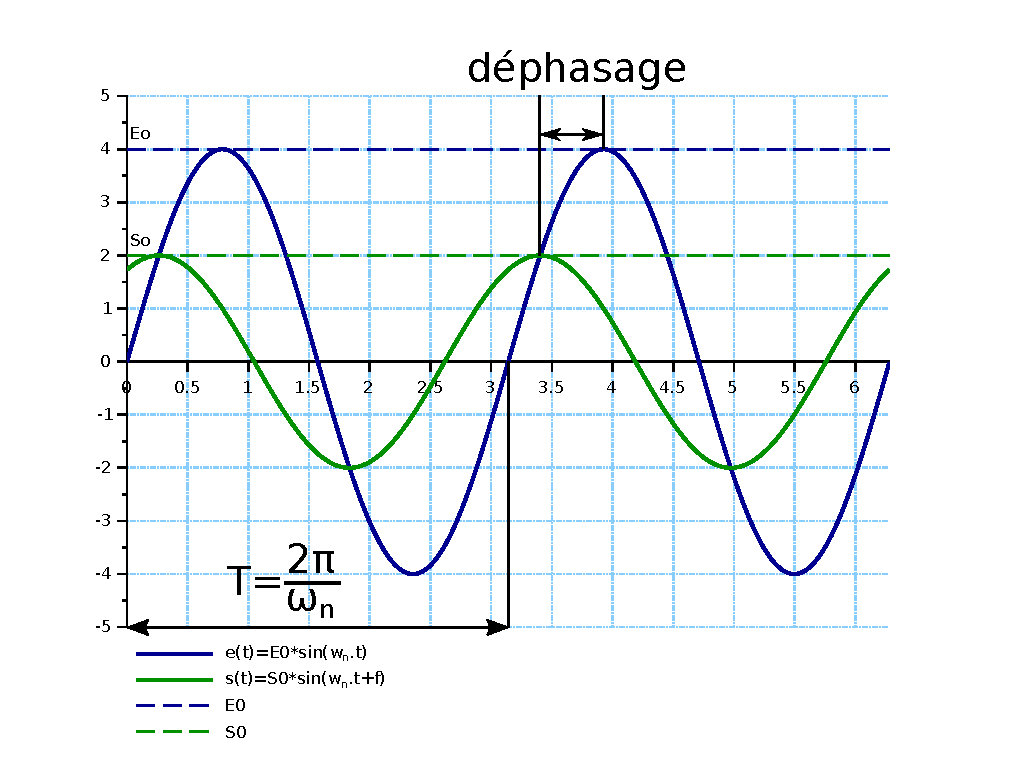
\includegraphics[width=0.5\linewidth]{img/harmo}
\end{center}

On appelle réponse harmonique, la sortie $s(t)$ en régime permanent d'un système soumis à une entrée $e(t)$ périodique. 
}}

{\frame{
\frametitle{Les diagrammes harmoniques}

Les courbes $e(t)$ et $s(t)$ dessinées ne sont valables que pour la pulsation $\omega_n$ du signal d'entrée. La représentation temporelle ne sera donc plus suffisante dans le cadre de cette étude.

\vfill

L'objet d'une étude fréquentielle d'un système est d'étudier l'évolution du \textbf{gain} et de la \textbf{phase}, en fonction de la variation de la valeur de la pulsation $\omega$ du signal d'entrée, sur la réponse harmonique du système.

\vfill

L'étude fréquentielle d'un système, consiste en l'étude, par la méthode des complexes, de la fonction de transfert du système H(p) : 
\begin{itemize}
 \item le \textbf{gain} du système $\frac{S_0}{E_0}$ qui est égal au module du nombre complexe $H(j\omega)$: $\frac{S_0}{E_0}=\vert H(j\omega) \vert$
 \item la \textbf{phase} du système $\varphi$ qui est égale à l'argument du nombre complexe $H(j\omega)$: $\varphi=arg(H(j\omega))$
\end{itemize}
}}


\section{Diagrammes de Bode}

{\frame{
\frametitle{Diagramme de Bode}

Plusieurs diagrammes permettent de décrire le comportement fréquentiel d'un système : Bode, Nyquist, Black. Dans un premier temps, nous nous limiterons à l'utilisation du diagramme de Bode.

Il est constitué de deux courbes correspondant aux tracés du module et la phase de $H(j\omega)$ en fonction de la pulsation sur une échelle logarithmique en base 10.

\vfill

\begin{minipage}{0.3\linewidth}
	\begin{itemize}
	 \item Le module $G_{db}=20\cdot log \vert H(j\omega) \vert$ est exprimé en décibel. 
	 \item La phase $\varphi$ est exprimée en degrés. 
	\end{itemize}
\end{minipage}
\hfill
\begin{minipage}{0.66\linewidth}
\centering
\def\svgwidth{0.75\columnwidth}
\input{img/bode1.pdf_tex}
\end{minipage}
}}

{\frame{
\frametitle{Cas du gain pur}

\begin{minipage}{0.48\linewidth}
\begin{center}
 \fbox{$H(p)=K$}
\end{center}
\end{minipage}
\hfill
\begin{minipage}{0.48\linewidth}
\begin{itemize}
 \item $G_{db}=20log\vert K \vert$  
 \item $\varphi=arg(K)=arctan\left(\dfrac{0}{K}\right)=0\textdegree$. 
\end{itemize}
\end{minipage}

\centering
\def\svgwidth{0.65\columnwidth}
\input{img/gain.pdf_tex}
}}

{\frame{
\frametitle{Cas de l'intégrateur}

\begin{minipage}{0.38\linewidth}
\begin{center}
 \fbox{$H(p)=\dfrac{K}{p}$}
\end{center}
\end{minipage}
\hfill
\begin{minipage}{0.58\linewidth}
\begin{itemize}
 \item $G_{db}=20log\bigg\vert \dfrac{K}{p} \bigg\vert=20log(K)-20log(\omega)$  
 \item $\varphi=arg\left(\dfrac{K}{j\omega}\right)=-arctan\left(\dfrac{\dfrac{\omega}{K}}{0}\right)=-90\textdegree$. 
\end{itemize}
\end{minipage}

\centering
\def\svgwidth{0.65\columnwidth}
\input{img/integrateur.pdf_tex}
}}

{\frame{
\frametitle{Cas du premier ordre}


\begin{minipage}{0.7\linewidth}
Pour $\omega \rightarrow 0$
\begin{itemize}
 \item $G_{db}=20log\bigg\vert \dfrac{K}{1+\tau.p} \bigg\vert=20log(K)-20log(1)=20log(K)$  
 \item $\varphi=arg\left(\dfrac{K}{1+\tau.j\omega}\right)=-arctan\left(\dfrac{0}{K}\right)=0\textdegree$.
 \end{itemize}
\end{minipage}\hfill
\begin{minipage}{0.27\linewidth}
\begin{center}
 \fbox{$H(p)=\dfrac{K}{1+\tau.p}$}
\end{center}
\end{minipage}
 
 Pour $\omega \rightarrow +\infty$
\begin{itemize}
 \item $G_{db}=20log\bigg\vert \dfrac{K}{1+\tau.p} \bigg\vert=20log\left(\dfrac{K}{\tau}\right)-20log(\omega)$  
 \item $\varphi=arg\left(\dfrac{K}{1+\tau.j\omega}\right)=-arctan\left(\dfrac{+ \infty}{K}\right)=-90\textdegree$. 
\end{itemize}

Pour $\omega=\omega_c=\dfrac{1}{\tau}$, pulsation de cassure.
\begin{itemize}
 \item $G_{db}=20log\left(\dfrac{K}{\sqrt{2}}\right)=20log(K)-3db$  
 \item $\varphi=arg\left(\dfrac{K}{1+\tau.j\omega_c}\right)=-arctan(1)=-45\textdegree$. 
\end{itemize}
}}

{\frame{
\frametitle{Cas du premier ordre}
\centering
\def\svgwidth{0.9\columnwidth}
\input{img/premier_ordre.pdf_tex}

}}

{\frame{
\frametitle{Cas du second ordre (z>1)}

\begin{center}
 \fbox{$H(p)=\dfrac{K}{1+\dfrac{2.z}{\omega_0}.p+\dfrac{p^2}{\omega_0^2}}$}
\end{center}

\textbf{Cas z>1}, alors $H(j\omega)=\dfrac{K}{(1+T_1.j.\omega).(1+T_2.j.\omega)}$

\vfill

\begin{itemize}
 \item $G_{db}=20log\bigg\vert \dfrac{K}{(1+T_1.j.\omega).(1+T_2.j.\omega)} \bigg\vert=20log(K)-10log(1+T_1^2.\omega^2))-10log(1+T_2^2.\omega^2))$  
 \item $\varphi=arg\left(\dfrac{K}{(1+T_1.j.\omega).(1+T_2.j.\omega)}\right)=-arctan\left(T_1.\omega\right)-arctan\left(T_2.\omega\right)$.
 \end{itemize}
 
Pour $\omega_0=\sqrt{\dfrac{1}{T_1.T_2}}$, la courbe de phase passe toujours par $-90\textdegree$.
}}

{\frame{
\frametitle{Cas du second ordre (z>1)}
\centering
\def\svgwidth{0.9\columnwidth}
\input{img/second_ordre_2.pdf_tex}

}}

{\frame{
\frametitle{Cas du second ordre (z=1)}

\begin{center}
 \fbox{$H(p)=\dfrac{K}{1+\dfrac{2.z}{\omega_0}.p+\dfrac{p^2}{\omega_0^2}}$}
\end{center}

\textbf{Cas z=1}, alors $H(j\omega)=\dfrac{K}{(1+T.j.\omega)^2}$

\vfill

\begin{itemize}
 \item $G_{db}=20log\bigg\vert \dfrac{K}{(1+T.j.\omega)^2} \bigg\vert=20log(K)-20log(1+T^2.\omega^2))$
 \item $\varphi=arg\left(\dfrac{K}{(1+T_1.j.\omega).(1+T_2.j.\omega)}\right)=-2.arctan\left(T.\omega\right)$.
 \end{itemize}
 
Pour $\omega_0=\sqrt{\dfrac{1}{T_1.T_2}}$, la courbe de phase passe toujours par $-90\textdegree$.
}}

{\frame{
\frametitle{Cas du second ordre (z=1)}
\centering
\def\svgwidth{0.9\columnwidth}
\input{img/second_ordre_1.pdf_tex}
}}


{\frame{
\frametitle{Cas du second ordre (z<1)}

\begin{center}
 \fbox{$H(p)=\dfrac{K}{1+\dfrac{2.z}{\omega_0}.p+\dfrac{p^2}{\omega_0^2}}$}
\end{center}

\textbf{Cas z<1}, alors $H(j\omega)=\dfrac{K}{1-\dfrac{\omega^2}{\omega_0^2}+j.\dfrac{2.z.\omega}{\omega_0}}$

\vfill

\begin{itemize}
 \item $G_{db}=20log\Bigg\vert \dfrac{K}{1-\dfrac{\omega^2}{\omega_0^2}+j.\dfrac{2.z.\omega}{\omega_0}} \Bigg\vert=20log(K)-10log\left(\left(1-\dfrac{\omega^2}{\omega_0^2}\right)^2+4.z^2.\left(\dfrac{\omega}{\omega_0}\right)^2\right)$
 \item $\varphi=arg\left(\dfrac{K}{1-\dfrac{\omega^2}{\omega_0^2}+j.\dfrac{2.z.\omega}{\omega_0}}\right)=
-arctan\left(\dfrac{\dfrac{2.z.\omega}{\omega_0}}{1-\dfrac{\omega^2}{\omega_0^2}}\right)$.
 \end{itemize}
}}

{\frame{
\frametitle{Cas du second ordre (z<1)}
\centering
\def\svgwidth{0.9\columnwidth}
\input{img/second_ordre.pdf_tex}
}}

{\frame{
\frametitle{Résonance}

Une résonance apparaît, lorsque $0<z<\dfrac{\sqrt{2}}{2}$, cela se manifeste par la présence d'un pic sur la courbe de gain.

Celui-ci étant un maximum, il peut être calculé s'il existe, pour la pulsation $\omega_r$ de la manière suivante: $\dfrac{dG}{d\omega}(\omega_r)=0$

\vfill

\begin{center}
$\left[\dfrac{d((\omega_0^2-\omega^2)^2+4.z^2\omega_0^2.\omega^2)}{d\omega}\right]_{\omega=\omega_r}=0$
\end{center}

\vfill

\begin{center}
$-4.\omega_r.(\omega_0^2-\omega_r^2)+8.z^2.\omega_0^2.\omega_r=0$.
\end{center}

\vfill

La résonance apparaît donc à la pulsation \fbox{$\omega_r=\omega_0.\sqrt{1-2.z^2}$}

\vfill

Et sa valeur est \fbox{$Q=\dfrac{|H(j.\omega)_{max}|}{|H(0)|}=\dfrac{1}{2.z.\sqrt{1-z^2}}$}.

}}

{\frame{
\frametitle{Conclusion}

\begin{savoir}
Vous êtes capables :
\begin{itemize}
 \item de construire les diagrammes de Bode à partir de fonctions de transfert,
 \item d'identifier des fonctions à partir de la lecture de ces diagrammes ou des tracés temporels.
\end{itemize}
\end{savoir}

\begin{prob}
Vous devez êtes capables :
 \begin{itemize}
 \item de mettre en place une correction de l'asservissement en vue du respect du cahier des charges.
 \end{itemize}
\end{prob}
}}


\end{document}